\documentclass[a4paper,12pt]{article} % добавить leqno в [] для нумерации слева
\usepackage[a4paper,top=1.3cm,bottom=2cm,left=1.5cm,right=1.5cm,marginparwidth=0.75cm]{geometry}
%%% Работа с русским языком
\usepackage{cmap}					% поиск в PDF
\usepackage{mathtext} 				% русские буквы в фомулах
\usepackage[T2A]{fontenc}			% кодировка
\usepackage[utf8]{inputenc}			% кодировка исходного текста
\usepackage[english,russian]{babel}	% локализация и переносы
\usepackage{multirow}

\usepackage{graphicx}

\usepackage{wrapfig}
\usepackage{tabularx}

\usepackage{hyperref}
\usepackage[rgb]{xcolor}
\hypersetup{
colorlinks=true,urlcolor=blue
}

%%% Дополнительная работа с математикой
\usepackage{amsmath,amsfonts,amssymb,amsthm,mathtools} % AMS
\usepackage{icomma} % "Умная" запятая: $0,2$ --- число, $0, 2$ --- перечисление

%% Номера формул
\mathtoolsset{showonlyrefs=true} % Показывать номера только у тех формул, на которые есть \eqref{} в тексте.

%% Шрифты
\usepackage{euscript}	 % Шрифт Евклид
\usepackage{mathrsfs} % Красивый матшрифт

%% Свои команды
\DeclareMathOperator{\sgn}{\mathop{sgn}}

%% Перенос знаков в формулах (по Львовскому)
\newcommand*{\hm}[1]{#1\nobreak\discretionary{}
{\hbox{$\mathsurround=0pt #1$}}{}}

%% Графики
\usepackage{tikz}
\usepackage{pgfplots}
\pgfplotsset{compat=1.9}

\date{\today}

\begin{document}

\begin{titlepage}
	\begin{center}
		{\large МОСКОВСКИЙ ФИЗИКО-ТЕХНИЧЕСКИЙ ИНСТИТУТ (НАЦИОНАЛЬНЫЙ ИССЛЕДОВАТЕЛЬСКИЙ УНИВЕРСИТЕТ)}
	\end{center}
	\begin{center}
		{\large Физтех-школа прикладной математики и информатики}
	\end{center}
	
	
	\vspace{4.5cm}
	{\huge
		\begin{center}
			{\bf Отчёт о выполнении лабораторной работы 3.2.1}\\
			Сдвиг фаз в цепи переменного тока
		\end{center}
	}
	\vspace{1cm}
	\begin{center}
		{\large Соболевский Федор Александрович \\
			\vspace{0.2cm}
			Б05-111}
	\end{center}
	\vspace{8cm}
	\begin{center}
		Сентябрь 2022
	\end{center}
\end{titlepage}

\section{Аннотация}

В данной работе исследованы вынужденные колебания в цепи переменного тока, вызываемые меняющейся по гармоническому закону ЭДС. Измерен сдвиг фаз между вызывающей колебания ЭДС и колебаниями тока в цепи, а также зависимость величины сдвига от активного сопротивления в цепи, индуктивности и ёмкости. 

\section{Теоретические сведения}

\subsection{Расчёт сдвига фаз в цепи переменного тока}

В цепи переменного тока, содержащей конденсаторы и/или катушки индуктивности, возникает сдвиг фаз между колебаниями тока в системе и вызывающей ЭДС. При подаче переменного тока на указанные элементы электрической цепи возникает реактивное сопротивление $X$, от величины которого и зависит сдвиг фаз. Выражение для сдвига фаз $\psi$ имеет вид

\begin{equation}
    \psi = 2\text{ arctg}\frac{X}{R_\Sigma},
\end{equation}

где $R_\Sigma$ - суммарное активное сопротивление цепи.

В зависимости от состава цепи реактивное сопротивление в ней рассчитывается разными способами. В RC-цепи реактивное сопротивление определяется как

\begin{equation}
    X_1 = 1/\omega C,
\end{equation}

где $\omega = 2\pi\nu$ - циклическая частота, $C$ - ёмкость конденсатора. Для RL выражение принимает вид

\begin{equation}
    X_2 = \omega L,
\end{equation}

где $L$ - индуктивность катушки. В случае RL-цепи в активном сопротивлении цепи также необходимо учесть активное сопротивление катушки $R_L$. 

В RLC-цепи сдвиг фаз зависит от соотношения частот генератора и частоты собственных колебаний контура. Сдвиг фаз равен $\psi = 0$ при резонансе контура и ЭДС. По формуле Томсона можно найти частоту резонанса:

\begin{equation}
    \nu_0 = 1/2\pi \sqrt{LC}.
\end{equation}

Комплексный импеданс RCL-цепочки:
$$Z=R+i\omega L - \frac{i}{\omega C}.$$

Сдвиг фаз между током и напряжением получим, взяв аргумент $Z$:

$$\tg\varphi = \frac{\omega L - \frac{1}{\omega C}}{R} = Q\frac{\left(\frac{\omega}{\omega_0}\right)^2 - 1}{\frac{\omega}{\omega_0}} = Q\frac{(1+x)^2-1}{1+x} \simeq 2x Q,$$

где $x = \Delta \omega / \omega_0 = \Delta \nu / \nu_0$. Измерив ширину $w=2x$ графика $|\psi|(\nu/\nu_0)$ на высоте $\varphi = \pi / 4\ (\tg\varphi = 1)$, можем непосредственно измерить добротность контура:

$$Q = \frac{1}{w}$$.

\subsection{Экспериментальная установка}

\begin{figure}
    \centering
    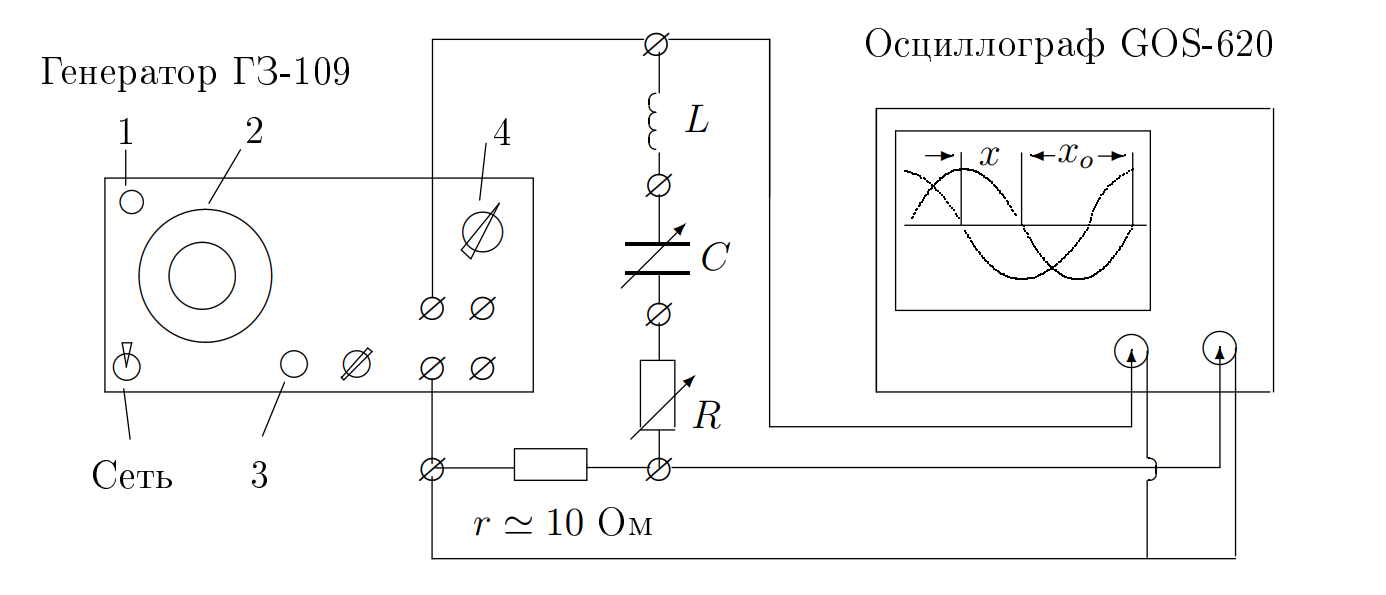
\includegraphics[width = 0.8\textwidth]{circuit1.png}
    \caption{Схема установки для исследования сдвига фаз между током и напряжением}
    \label{fig:circuit1}
\end{figure}

На рис. \ref{fig:circuit1} изображена схема RCL-цепи, используемой для измерения сдвига фаз между током и напряжением. В качестве источника синусоидального напряжения используется звуковой генератор. С сопротивления $r$ снимается сигнал, пропорциональный току, со звукогенератора - пропорциональный напряжению. Оба сигнала подаются на универсальный осциллограф, имеющий два канала вертикального отклонения. При этом на экране ЭО видны две синусоиды, смещённые друг относительно друга на некоторое расстояние $x$, из которого и можно найти сдвиг фаз.

\begin{figure}
    \centering
    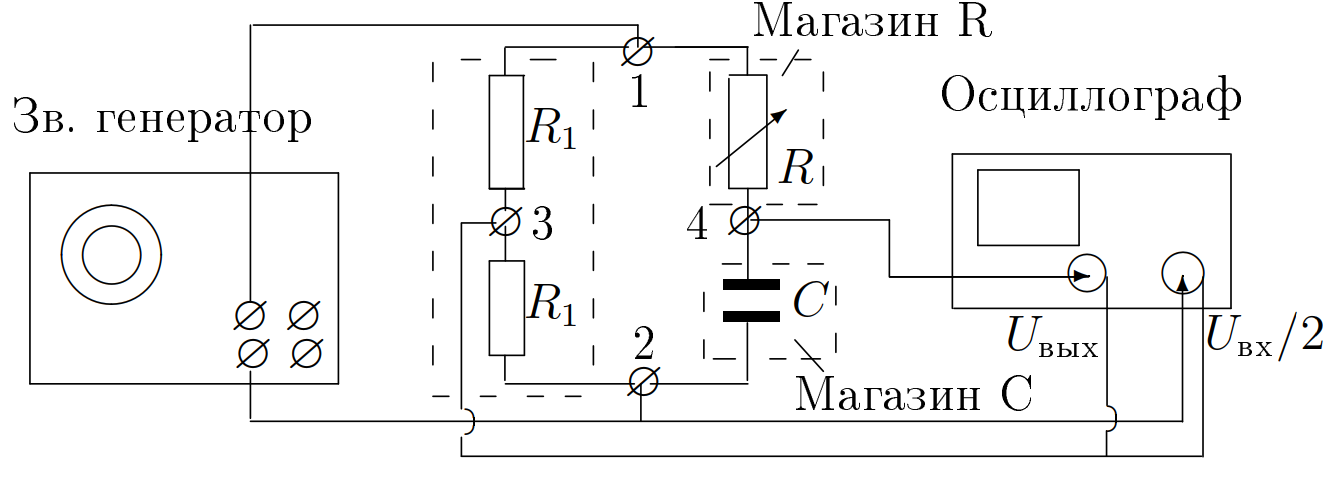
\includegraphics[width = 0.8\textwidth]{circuit2.png}
    \caption{Схема установки для исследования фазовращателя}
    \label{fig:circuit2}
\end{figure}

Для изменения фазы напряжения в работе был применён фазовращатель - прибор, позволяющий менять фазу напряжения в широких пределах ($0 < \psi < \pi$). Схема цепи с фазовращателем изображена на рис. \ref{fig:circuit2}. Она содержит два одинаковых резистора $R_1$, магазин сопротивлений $R$ и магазин ёмкостей $C$.

Выражение для сдвига фаз между входным и выходным напряжениями имеет вид

$$\psi = \arg \frac{U_\text{вых}}{U_\text{вх}} = 2 \text{ arctg} \frac{1}{\omega RC} $$,

где $U_\text{вых}$ и $U_\text{вх}$ - выходное и входное напряжения соотвественно.

\section{Оборудование и инструментальные погрешности}

\textbf{В работе использовались:} генератор звуковой частоты, двухканальный электронный осциллограф, магазин ёмкостей, магазин сопротивлений, эталонная катушка индуктивности, резисторы.

Относительные систематические погрешности всех измерительных приборов в силу их высокой точности примем равными $\delta = 0,01$.

\section{Результаты измерений и обработка экспериментальных данных}

Показания лабораторных приборов: $C = 0,5$ мкФ, $\nu = 1000$ Гц, $L = 50$ мГн, $r = 12,2$ Ом, $R_L = 31$ Ом. 

\subsection{Измерение сдвига фаз в RC- и RL-цепях}

Реактивное сопротивление в RC-цепи $X_1 = 1/(2\pi \nu C) = 318 \pm 5$ Ом, в RL-цепи - $X_2 = 2\pi\nu L = 314 \pm 5$ Ом. Суммарное активное сопротивление в RC-цепи $R_\Sigma = R + r$, в RL-цепи - $R_\Sigma = R + r + R_L$. Результаты измерения сдвига фаз в данных цепях в зависимости от сопротивления магазина $R$ представлены в таблицах \ref{tab:RC} и \ref{graph:RL} и на графиках \ref{graph:RC} и \ref{graph:RL}.

\begin{table}
\centering
\begin{tabular}{|c|c|c|c|c|c|c|c|}
\hline
$R, \text{ Ом}$ & $x$ & $x_0$ & $\psi$ & $\ctg \psi$ & $R_{\Sigma}, \text{ Ом}$ & $R_{\Sigma} \omega C$ & $\sigma_{\ctg\psi}$\\ \hline
0&	    0&	    19.0&	    0&	    -&	    43,2&	0.14&	-\\ \hline
500&	13.0&  	19.0&	    2.1&	0.65&	543,2&	1.71&	0,23\\ \hline
1000&	17.0&	20.0&	    2.7&	1.96&	1043,4&	3.28&	0,20\\ \hline
1500&	18.0&	20.5&	    2.8&	2.48&	1543,4&	4.85&	0,02\\ \hline
2000&	19.0&  	21.0&	    2.8&	3.24&	2043,4&	6.42&	0,01\\ \hline
2500&	19.2&  	21.0&	    2.8&	3.73&	2543,4&	7.99&	0,07\\ \hline
3000&	19.5&  	21.0&   	2.9&	4.38&	3043,4&	9.56&	0,08\\ \hline
\end{tabular}
\caption{Результаты измерения сдвига фаз в RC-цепи}
\label{tab:RC}
\end{table}

\begin{table}
\centering
\begin{tabular}{|c|c|c|c|c|c|c|c|}
\hline
$R, \text{ Ом}$ & $x$ & $x_0$ & $\psi$ & $\ctg \psi$ & $R_{\Sigma}, \text{ Ом}$ & $R_{\Sigma}/( \omega L)$ & $\sigma_{\ctg\psi}$\\ \hline
0&	    18&	    19&	    0&	    -&	    12,2&	0.04&	-\\ \hline
500&	6&  	19&	    2.0&	0.44&	512,2&	1.61&	0,45\\ \hline
1000&	3,5&	19&	    2.6&	1.53&	1012,4&	3.18&	0,04\\ \hline
1500&	2,5&	19&	    2.7&	2.28&	1512,4&	4.75&	0,04\\ \hline
2000&	2&  	19&	    2.8&	2.91&	2012,4&	6.32&	0,08\\ \hline
2500&	1&  	19&	    2.9&	3.95&	2512,4&	7.89&	0,01\\ \hline
3000&	0,5&  	19& 	3.0&	5.99&	3012,4&	9.46&	0,27\\ \hline
\end{tabular}
\caption{Результаты измерения сдвига фаз в RL-цепи}
\label{tab:RL}
\end{table}

\begin{figure}
\centering
\resizebox {0.55\textwidth} {!} {
\begin{tikzpicture}
\begin{axis}[ xlabel = {$R_{\Sigma} \omega C$}, ylabel = {$\ctg \psi$}, xmin = 0, xmax = 10, ymin = 0, ymax = 6]
\addplot[color=black, mark=x, only marks] coordinates{
(1.71, 0.65)
(3.28, 1.96)
(4.85, 2.48)
(6.42, 3.24)
(7.99, 3.73)
(9.56, 4.38)
};
\addplot[color=blue, domain=0:10] {0.5*x};
\legend{Эксп., Теор.}
\end{axis}
\end{tikzpicture}
}
\caption{График зависимости сдвига фаз от сопротивления в RC-цепи}
\label{graph:RC}
\end{figure}

\begin{figure}
\centering
\resizebox {0.55\textwidth} {!} {
\begin{tikzpicture}
\begin{axis}[ xlabel = {$R_{\Sigma}/( \omega L)$}, ylabel = {$\ctg \psi$}, xmin = 0, xmax = 10, ymin = 0, ymax = 6]
\addplot[color=black, mark=x, only marks] coordinates{
(1.61, 0.44)
(3.18, 1.53)
(4.75, 2.28)
(6.32, 2.91)
(7.89, 3.95)
(9.46, 5.99)
};
\addplot[color=blue, domain=0:10] {0.5*x};
\legend{Эксп., Теор.}
\end{axis}
\end{tikzpicture}
}
\caption{График зависимости сдвига фаз от сопротивления в RL-цепи}
\label{graph:RL}
\end{figure}

\subsection{Фазово-частотная характеристика RCL-цепи}

Для значение сопротивления магазина $R = 0$ и $R = 100$ Ом были измерены сдвиги фаз при изменении частоты звукогенератора относительно резонансной. Резонансная частота $\nu_0 = 1/(2\pi\sqrt{LC}) = 1007 \pm 14$ Гц. Результаты измерений в RCL-цепи представлены в таблице \ref{tab:RCL}. По полученным данным построена фазово-частотная характеристика цепи, представленная на рис. \ref{graph:RСL}. 

\begin{table}
\centering
\begin{tabular}{|c|c|c|c|c|c|}
\hline
$R$, Ом & $\nu, \text{Гц}$ & $x$ & $x_0$ & $\nu/\nu_0$ & $|\psi|$ \\ \hline
\multirow{11}{*}{0}   
&1020	&0		&4,9	&1,013	&0,000	\\ \cline{2-6}
&1000	&0,4	&4,9	&0,993	&0,256	\\ \cline{2-6} 
&980	&0,9	&5,2	&0,974	&0,544	\\ \cline{2-6} 
&960	&1,2	&5,2	&0,954	&0,725	\\ \cline{2-6} 
&940	&1,5	&5,3	&0,934	&0,889	\\ \cline{2-6} 
&930	&1,7	&5,4	&0,924	&0,989	\\ \cline{2-6}
&1040	&0,8	&4,9	&1,033	&0,513	\\ \cline{2-6} 
&1060	&1,1	&4,9	&1,053	&0,705	\\ \cline{2-6} 
&1080	&1,3	&4,7	&1,073	&0,869	\\ \cline{2-6} 
&1100	&1,5	&4,8	&1,093	&0,982	\\ \cline{2-6} 
&1120	&1,6	&4,5	&1,113	&1,117	\\ \hline 
\multirow{11}{*}{100} 
&1020	&0		&4,8	&1,013	&0,000	\\ \cline{2-6}
&1000	&0,1	&5,0	&0,993	&0,063	\\ \cline{2-6}
&980	&0,2	&5,2	&0,974	&0,121	\\ \cline{2-6}
&960	&0,4	&5,3	&0,954	&0,237	\\ \cline{2-6}
&940	&0,5	&5,3	&0,934	&0,296	\\ \cline{2-6}
&930	&0,6	&5,4	&0,924	&0,349	\\ \cline{2-6}
&1040	&0,2	&4,9	&1,033	&0,128	\\ \cline{2-6}
&1060	&0,3	&4,7	&1,053	&0,201	\\ \cline{2-6}
&1080	&0,4	&4,6	&1,073	&0,273	\\ \cline{2-6}
&1100	&0,5	&4,6	&1,093	&0,341	\\ \cline{2-6}
&1120	&0,6	&4,5	&1,113	&0,419	\\ \hline 
\end{tabular}
\caption{Зависимость сдвига фаз от частоты в RCL-цепи}
\label{tab:RCL}
\end{table}

\begin{figure}
\centering
\resizebox {0.55\textwidth} {!} {
\begin{tikzpicture}
\begin{axis}[ xlabel = {$\nu/\nu_0$}, ylabel = {$\psi$}, xmin = 0.75, xmax = 1.25, ymin = 0, ymax = 1.3]
\addplot[color=black, mark=o, only marks] coordinates{
(1.013, 0)
(0.993, 0.256)
(0.974, 0.544)
(0.954, 0.725)
(0.934, 0.889)
(0.924, 0.989)
(1.033, 0.513)
(1.053, 0.705)
(1.073, 0.869)
(1.093, 0.982)
(1.113, 1.117)
};
\addplot[color=black, mark=x, only marks] coordinates{
(1.013, 0)
(0.993, 0.063)
(0.974, 0.121)
(0.954, 0.237)
(0.934, 0.296)
(0.924, 0.349)
(1.033, 0.128)
(1.053, 0.201)
(1.073, 0.273)
(1.093, 0.341)
(1.113, 0.419)
};
\addplot[color=blue, domain=0:10] {3.1415/4 + x - x};
\legend{$R = 0$, $R = 100 Ом$, $\psi = \pi/4$}
\addplot[color=red] coordinates{
(0.93, 0.989)
(1.013, 0)
(1.07, 1.117)
};
\addplot[color=red] coordinates{
(0.791, 0.825)
(1.013, 0)
(1.213, 0.838)
};
\end{axis}
\end{tikzpicture}
}
\caption{Фазово-частотная характеристика RCL-цепи}
\label{graph:RСL}
\end{figure}

С помощью графика можно найти добротность цепи $Q$, измерив ширину кривой при сдвиге фаз $\psi = \pi/4$:

$$ Q = \frac{\nu_0}{2\Delta\nu}$$.

Также добротность можно рассчитать через параметры контура $R_\Sigma$, $C$ и $L$:

$$Q = \frac{1}{R_\Sigma} \sqrt{\frac{L}{C}}$$

Результаты измерения добротности следующие:

\begin{itemize}
    \item $R = 0$: $Q_{0} = 7.7 \pm 0.6$, $Q_{\text{теор, 0}} = 7.3 \pm 0.3$
    \item $R = 100$ Ом: $Q_{100} = 2.3 \pm 0.5$, $Q_{\text{теор, 100}} = 2.2 \pm 0.2$
\end{itemize}

Видно, что значения добротности совпадают с теоретическими в пределах погрешности измерений.

\subsection{Измерения с помощью фазовращателя}

\begin{figure}
    \centering
    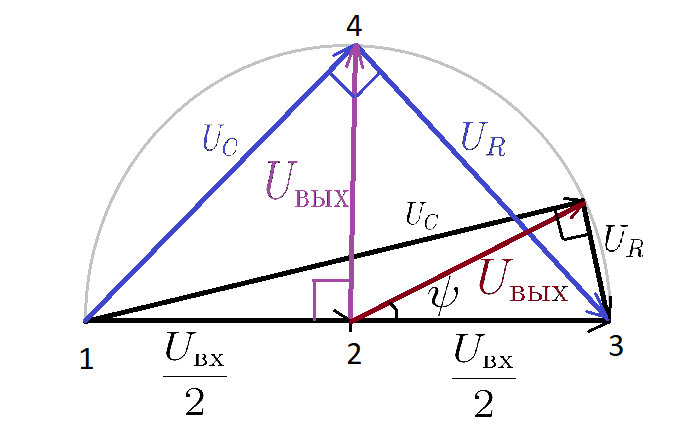
\includegraphics[width = 0.7\textwidth]{diagram.png}
    \caption{Векторная диаграмма для фазовращателя}
    \label{fig:diagram}
\end{figure}

Векторная диаграмма для фазовращателя представлена на рис. \ref{fig:diagram}. На ней видно, что сдвиг фаз между входным и выходным напряжением равен $\pi/2$, когда реактивное и активное сопротивления $X_C$ и $R$ равны по модулю, т.е. $R$ равно рассчитанному ранее $X_1 = 318$ Ом. В ходе эксперимента было установлено, что сдвиг фаз $\psi = \pi/2$ достигается при сопротивлении магазина, равном 310 Ом, что близко к теоретическому значению.

\section{Обсуждение результатов и выводы}

В данной работе представилось возможным зафиксировать сдвиг фаз в цепи переменного тока. Зависимость данного сдвига в эксперименте совпала с теоретической в пределах требуемой точности измерений. Это позволяет утверждать, что теоретические закономерности выполняются в лабораторных условиях с достаточной точностью при измерениях в диапазоне от ~10 до ~10$^3$ Ом.

Добротность исследованной RCL-цепи не превысила 10 при нулевом сопротивлении магазина, а при подключении дополнительного сопротивления и вовсе близка к единице. Это позволяет сделать вывод о том, что данная установка мало подходит для изучения собственных слабозатухающих колебаний в RCL-цепи, так как затухание колебаний в такой цепи будет слишком быстрым (меньше 1 секунды). Однако проведённый опыт показал, что полученные значения добротности установки достаточны для применимости использованной установки при исследовании вынужденных колебаний.

\end{document}
